%\documentclass[pdftex,a4paper,12pt]{article}
%\linespread{1.1}
%\usepackage[english,german,ngerman]{babel}
%\usepackage[utf8]{inputenc}
%\usepackage[T1]{fontenc}
%%\usepackage{lmodern}
%%\usepackage{amsfonts}
%\usepackage{iwona}
%
%
%\usepackage{graphicx}
%\usepackage{hyperref}
%\usepackage[export]{adjustbox}
%
\newcommand\winkey{
\includegraphics[height=1em]{imgs/Windows_logo_-_2006.eps}}
\newcommand\tbs\textbackslash
%
%{
%\catcode`\^0
%\catcode`\\12
%^gdef^dirsep{\}
%}
%
%\title{Installationsanleitung \\
%f�r Eclipse CDT und Cygwin \\
%(auf Windows)}
%\author{Tobias G�dderz}
%\date{28.9.2013}
%
%\begin{document}
%
%\maketitle

\subsection{Architektur (32bit oder 64bit?)}

Ihr solltet f�r die Installation wissen, ob ihr ein 32- oder 64bit Windows
installiert habt. Wenn ihr das nicht bereits tut, k�nnt ihr es nachsehen, wenn
ihr \texttt{\winkey+R} dr�ckt und dort ``\texttt{control /name
Microsoft.System}'' eingebt. Dort steht zum Beispiel ``\textit{System type:
64-bit Operating System}''.

Auf 64bit Betriebssystemen k�nnt ihr auch 32bit Software benutzen, aber nicht
andersherum.

\subsection{Java}

F�r Eclipse m�sst ihr eine Java Runtime Environment installieren. Wenn ihr
32bit-Eclipse verwenden wollt, braucht ihr die 32bit Version der JRE. Wenn ihr
64bit-Eclipse verwenden wollt, braucht ihr die 64bit Version der JRE. Ihr k�nnt
auch beide Varianten der JRE installieren. Ihr findet beide hinter folgendem
Link: \url{http://www.java.com/en/download/}

\pagebreak

\begin{center}
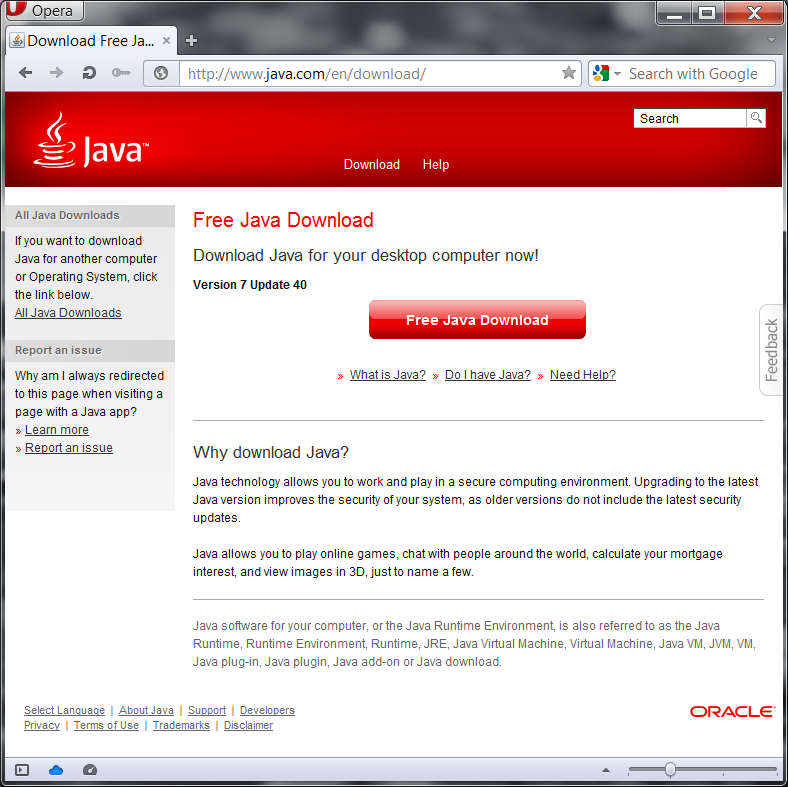
\includegraphics[scale=.4]{imgs/java-homepage-1.png}
\end{center}

\begin{center}
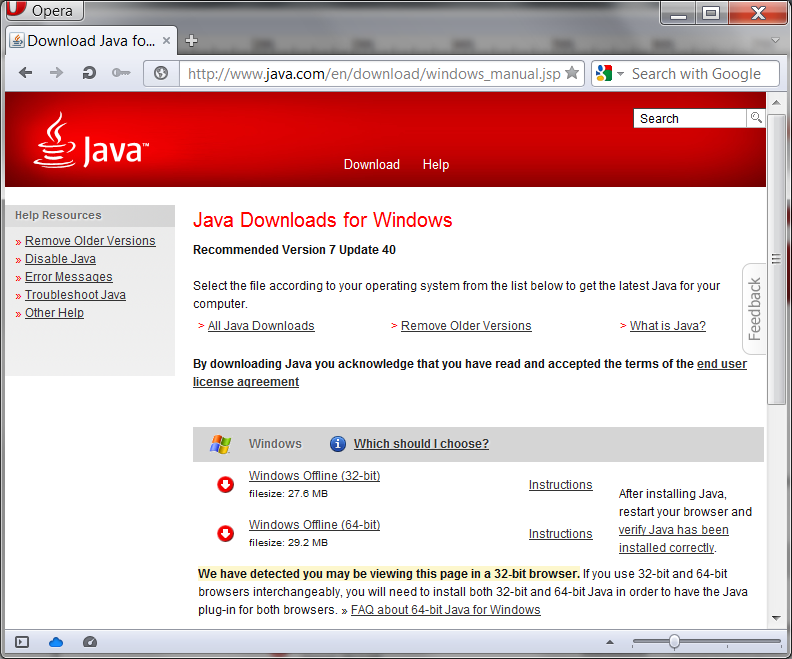
\includegraphics[scale=.4]{imgs/java-homepage-2.png}
\end{center}

\subsection{Cygwin}

Das Cygwin Setup k�nnt ihr auf \url{http://cygwin.org/} herunterladen.

\begin{center}
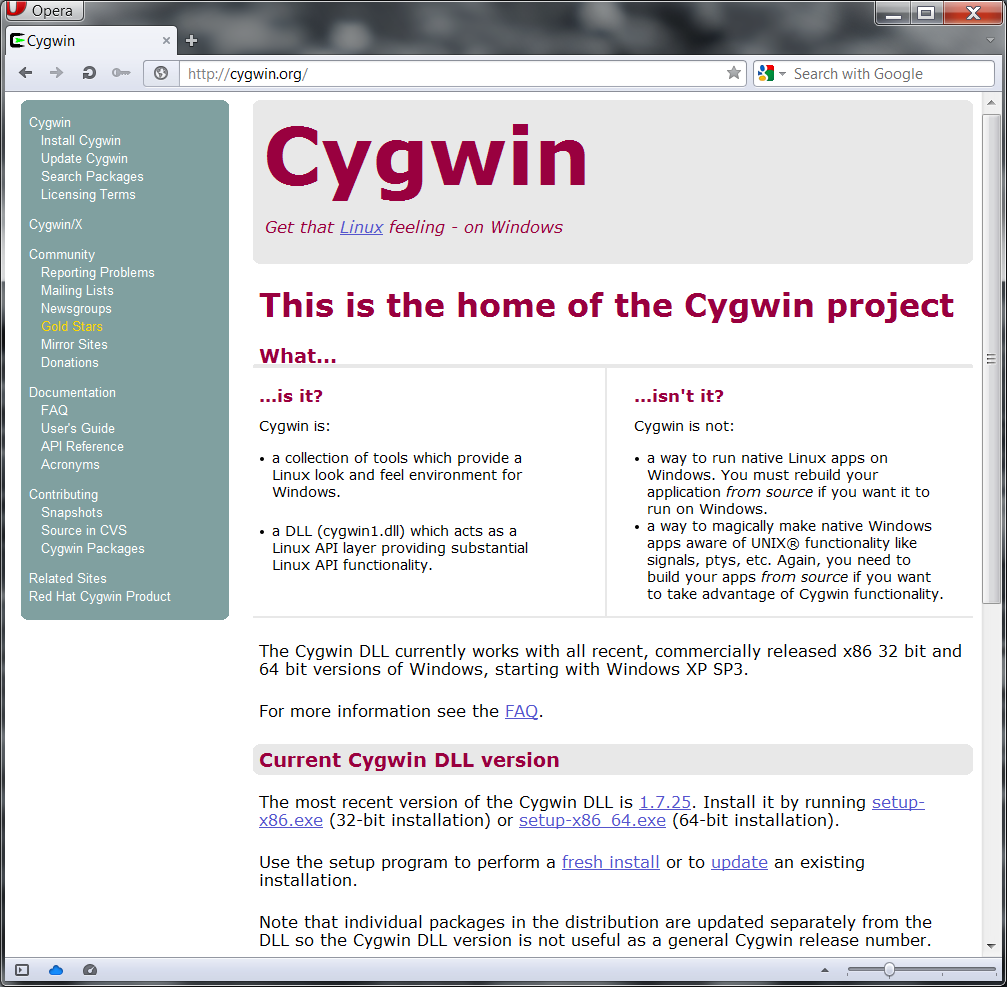
\includegraphics[scale=.4,max width=.9\textwidth]{imgs/cygwin-homepage.png}
\end{center}

Es ist wichtig, Cygwin in einen Pfad ohne Leerzeichen o.�.\ zu installieren.
Belasst es also bitte bei dem empfohlenen Installationspfad
\texttt{C:\tbs{}cygwin} bzw.  \texttt{C:\tbs{}cygwin64}.  W�hrend der
Installation w�hlt ihr bitte die folgenden Pakete aus:

\begin{itemize}
    \item gcc-core
    \item gdb
    \item make
\end{itemize}

\subsubsection{PATH setzen}

Danach m�sst ihr Cygwin zu der Umgebungsvariable PATH hinzuf�gen, damit eclipse
die ben�tigten Programme findet. Daf�r dr�ckt ihr \texttt{\winkey+R} und gebt
``\texttt{control sysdm.cpl,,3}'' (sic) ein. Es �ffnet sich ein Fenster
\textit{System Properties}.

\begin{center}
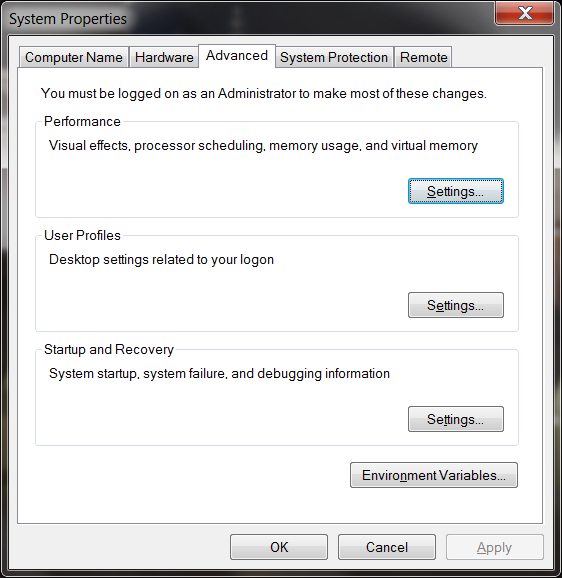
\includegraphics[scale=.4]{imgs/system_properties-advanced.png}
\end{center}

Dort klickt ihr auf \texttt{Environment Variables}.

\begin{center}
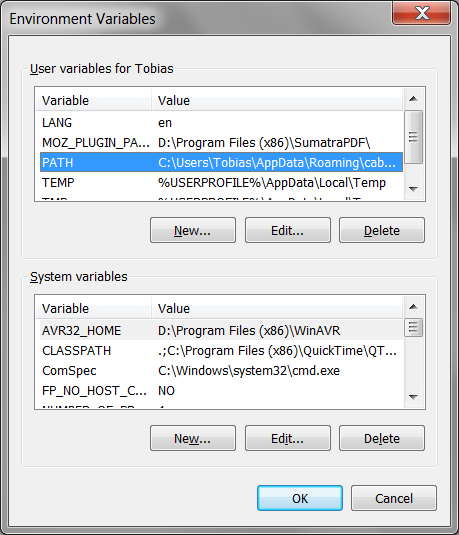
\includegraphics[scale=.4]{imgs/system_properties-advanced-env.png}
\end{center}

Schaut bitte oben unter \textit{User variables} nach, ob dort bereits eine
Variable mit dem Namen PATH existiert. Falls nicht, legt ihr eine neue Variable
mit dem Namen PATH und dem Wert ``\texttt{C:\tbs{}cygwin64\tbs{}bin}'' an (falls
ihr Cygwin in \texttt{C:\tbs{}cygwin64} installiert habt, sonst passt den Pfad
bitte entsprechend an). Falls die Variable bereits existiert, editiert ihr sie,
bewegt den Cursor ganz ans Ende des Textes (z.B.\ indem ihr auf eure
\texttt{Ende} Taste dr�ckt) und f�gt dort den gleichen Pfad ein, aber
\textit{mit einem Semikolon von dem existierenden getrennt}, also z.B.
``\texttt{;C:\tbs{}cygwin64\tbs{}bin}''.

\begin{center}
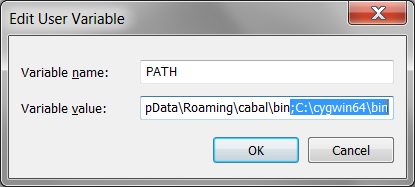
\includegraphics[scale=.4]{imgs/system_properties-advanced-env-set.png}
\end{center}

\subsection{Eclipse CDT}

Eclipse findet ihr auf \url{http://www.eclipse.org/downloads/}.

\begin{center}
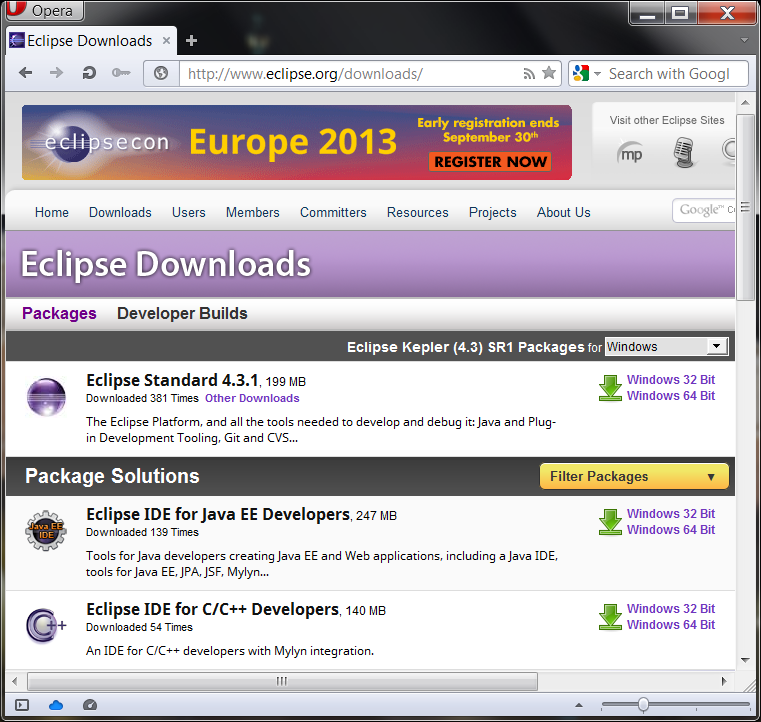
\includegraphics[scale=.4]{imgs/eclipse-homepage.png}
\end{center}

Ihr m�sst dort die \textit{Eclipse IDE for C/C++ Developers} herunterladen (und
nicht etwa \textit{Eclipse Standard}). Ladet die \texttt{.zip} Datei herunter
und extrahiert sie an einen Ort eurer Wahl. Empfehlenswert ist
``\texttt{C:\tbs{}Program Files}'' oder, wenn ihr 32bit-Eclipse auf einem 64-bit
Betriebssystem verwendet, ``\texttt{C:\tbs{}Program Files (x86)}''.

Nachdem ihr es entpackt habt k�nnt ihr es einfach starten. Legt euch einen Pfad
f�r den Workspace \textit{ohne Leerzeichen} an und klickt auf \textrm{OK}.
 
\begin{center}
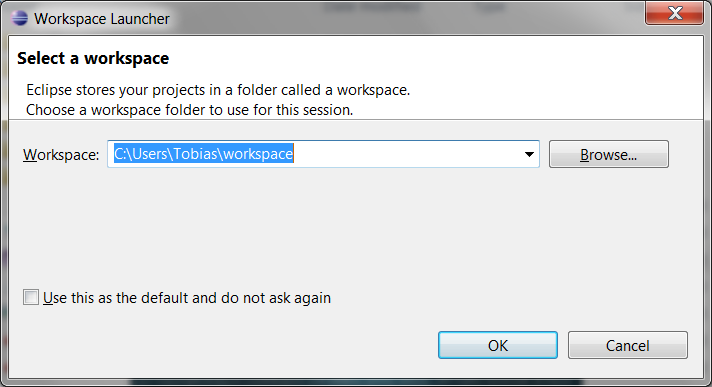
\includegraphics[scale=.4]{imgs/eclipse-workspace_launcher.png}
\end{center}

Auf dem \textit{Welcome}-Bildschirm m�sst ihr dann auf ``Workbench'' klicken
(der Button rechts).

\begin{center}
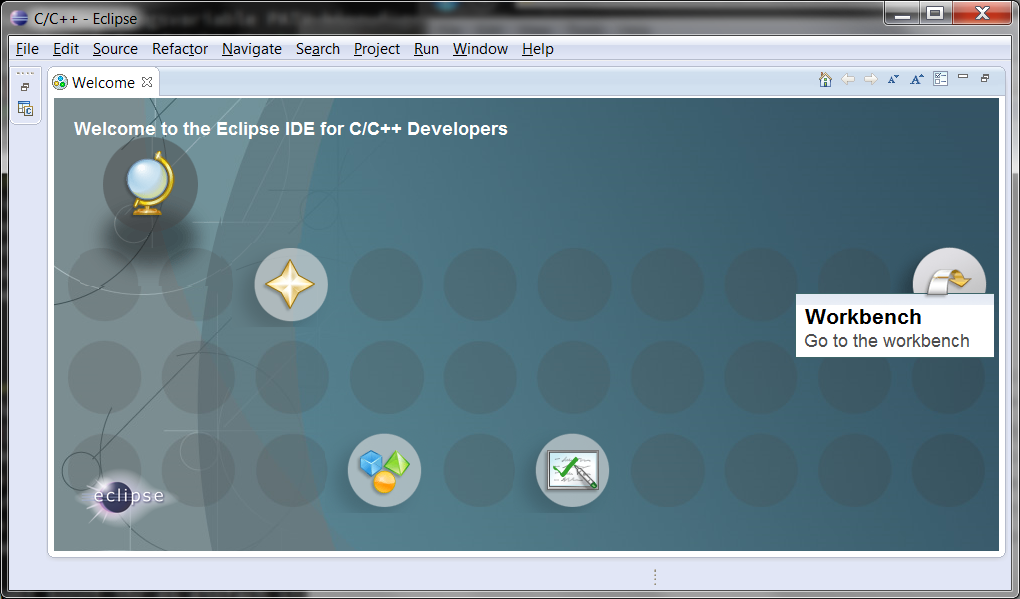
\includegraphics[scale=.4]{imgs/eclipse-welcome.png}
\end{center}

Legt dort ein neues C-Projekt an.

\begin{center}
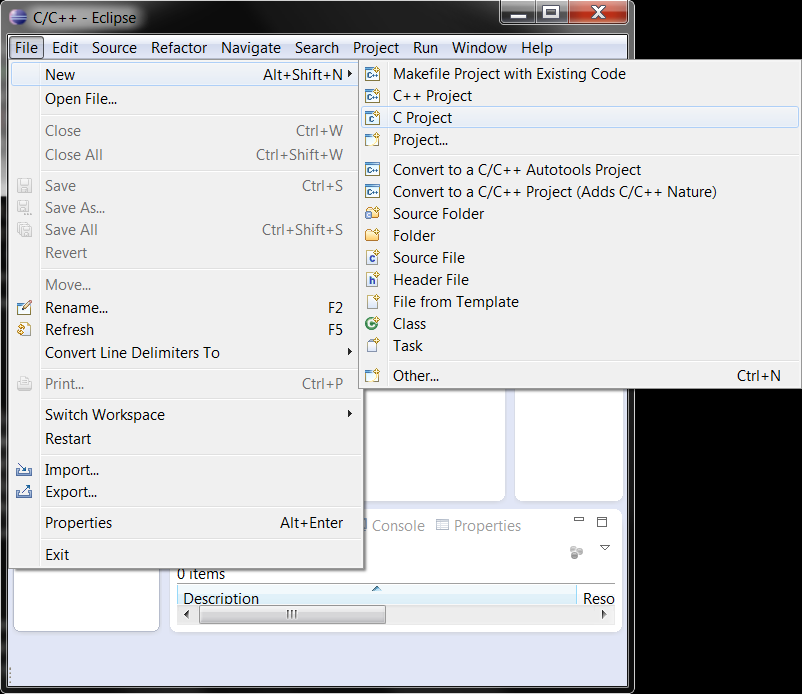
\includegraphics[scale=.4]{imgs/eclipse-new_c_project.png}
\end{center}

W�hlt einen Projektnamen \textit{ohne Leerzeichen}. Zum ersten Testen w�hlt das
``Hello World ANSI C Project'', ansonsten ``Empty Project''. Beim Hello-World
Projekttyp wird direkt eine \texttt{.c} Datei generiert, die ihr ausprobieren
k�nnt. Jetzt w�hlt die Cygwin GCC Toolchain aus (Vorsicht: wenn ihr danach den
Projekttyp wechselt, �ndert sich die gew�hlte Toolchain wieder).

\begin{center}
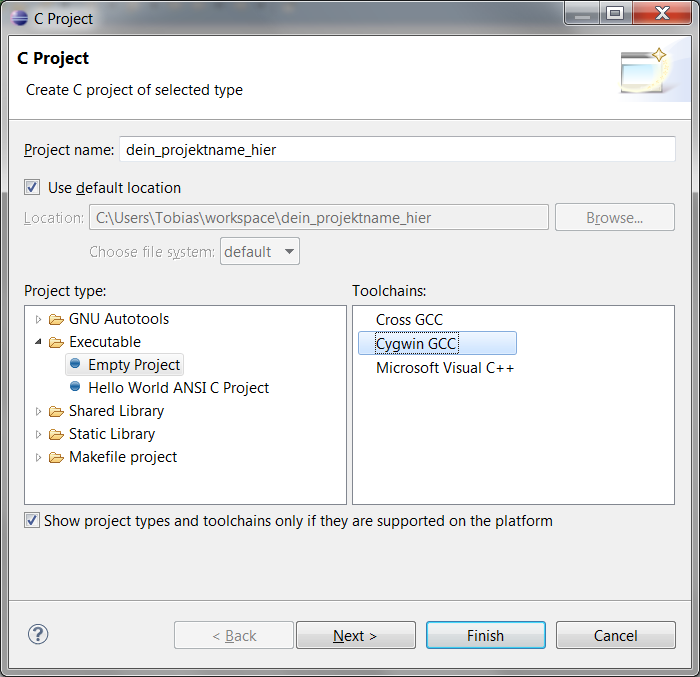
\includegraphics[scale=.4]{imgs/eclipse-c_project.png}
\end{center}

Kompiliert das Projekt, indem ihr das Build-Icon

\includegraphics[height=1em]{imgs/eclipse-icon-build.png} anklickt.  F�hrt das
kompilierte Programm aus, indem ihr auf

\includegraphics[height=1em]{imgs/eclipse-icon-run.png} klickt.

Viel Spa�!

%\end{document}
